\documentclass[a4]{article}
\usepackage{amssymb}
\usepackage{amsmath}
\usepackage{listings}
\usepackage{graphicx}
\usepackage{../../manual/manual}
\newcounter{lst}[section]

\renewcommand{\thelst}{\arabic{section}.\arabic{lst}}

\lstset{basicstyle=\footnotesize\sffamily}

\lstdefinestyle{easslisting}{basicstyle=\footnotesize\sffamily, mathescape=true, frame=tb,  numbers=right, numberstyle=\footnotesize, stepnumber=1, numbersep=-5pt, captionpos=b}

\lstdefinestyle{eass}{basicstyle=\sffamily, mathescape=true}

\lstnewenvironment{listing}[3]{
  \noindent        
  \refstepcounter{lst}         
  \label{code:#1}  
\begin{tabular}{p{.97\columnwidth}} \\ \hline  {\normalsize \textbf{Code  fragment \arabic{section}.\arabic{lst}} #2} \\  \end{tabular} 
\lstset{language=#3,          
  basicstyle=\footnotesize\sffamily,
%%%  basicstyle=\footnotesize,    
  xleftmargin=10pt,    
  mathescape=true,    
  frame=tb,    
  numbers=right,    
%%%  numberstyle=\tiny,     
  numberstyle=\footnotesize,     
  stepnumber=1,     
  numbersep=-5pt}}{}

%-- definition for Gwendolen --%

\lstdefinelanguage{Gwendolen}{%
    morekeywords={Plans,Initial,Beliefs,Goals,name,fof-parse,Rules,Belief,Reasoning},
    morecomment=[l]{//},
 literate= {<-}{{$\leftarrow$}{$\:$}}2
           {.B}{{${\cal B}$}}2
           {.G}{{${\cal G}$}}2
           {lnot}{{$\sim$}}2
           {assert_shared}{{$+_{\Sigma}$}}2
           {remove_shared}{{$-_{\Sigma}$}}2
           {(perform)}{}0
}



\makeindex

\author{Louise A. Dennis}

\title{Gwendolen Tutorial 7 -- The Gwendolen Reasoning Cycle}

\begin{document}
\maketitle
This is the seventh in a series of tutorials on the use of the \gwendolen\ programming language.  This tutorial covers the \gwendolen\ Reasoning Cycle, looks at some simple ways to use a Java Debugger to debug \gwendolen\ programs and sets a more significant programming challenge than previous tutorials.

Files for this tutorial can be found in the \texttt{mcapl} distribution in the directory \texttt{src/examples/gwendolen/tutorials/tutorial7}.

\section{The \gwendolen\ Reasoning Cycle}

The execution of a \gwendolen\ agent is governed by a \emph{reasoning cycle}.  This is a set of stages the agent passes through, each stage is governed by a set of rules and the agent may choose one to execute in that stage.  The reasoning cycle is shown in figure~\ref{fig:reasoning_cycle}
\begin{figure}
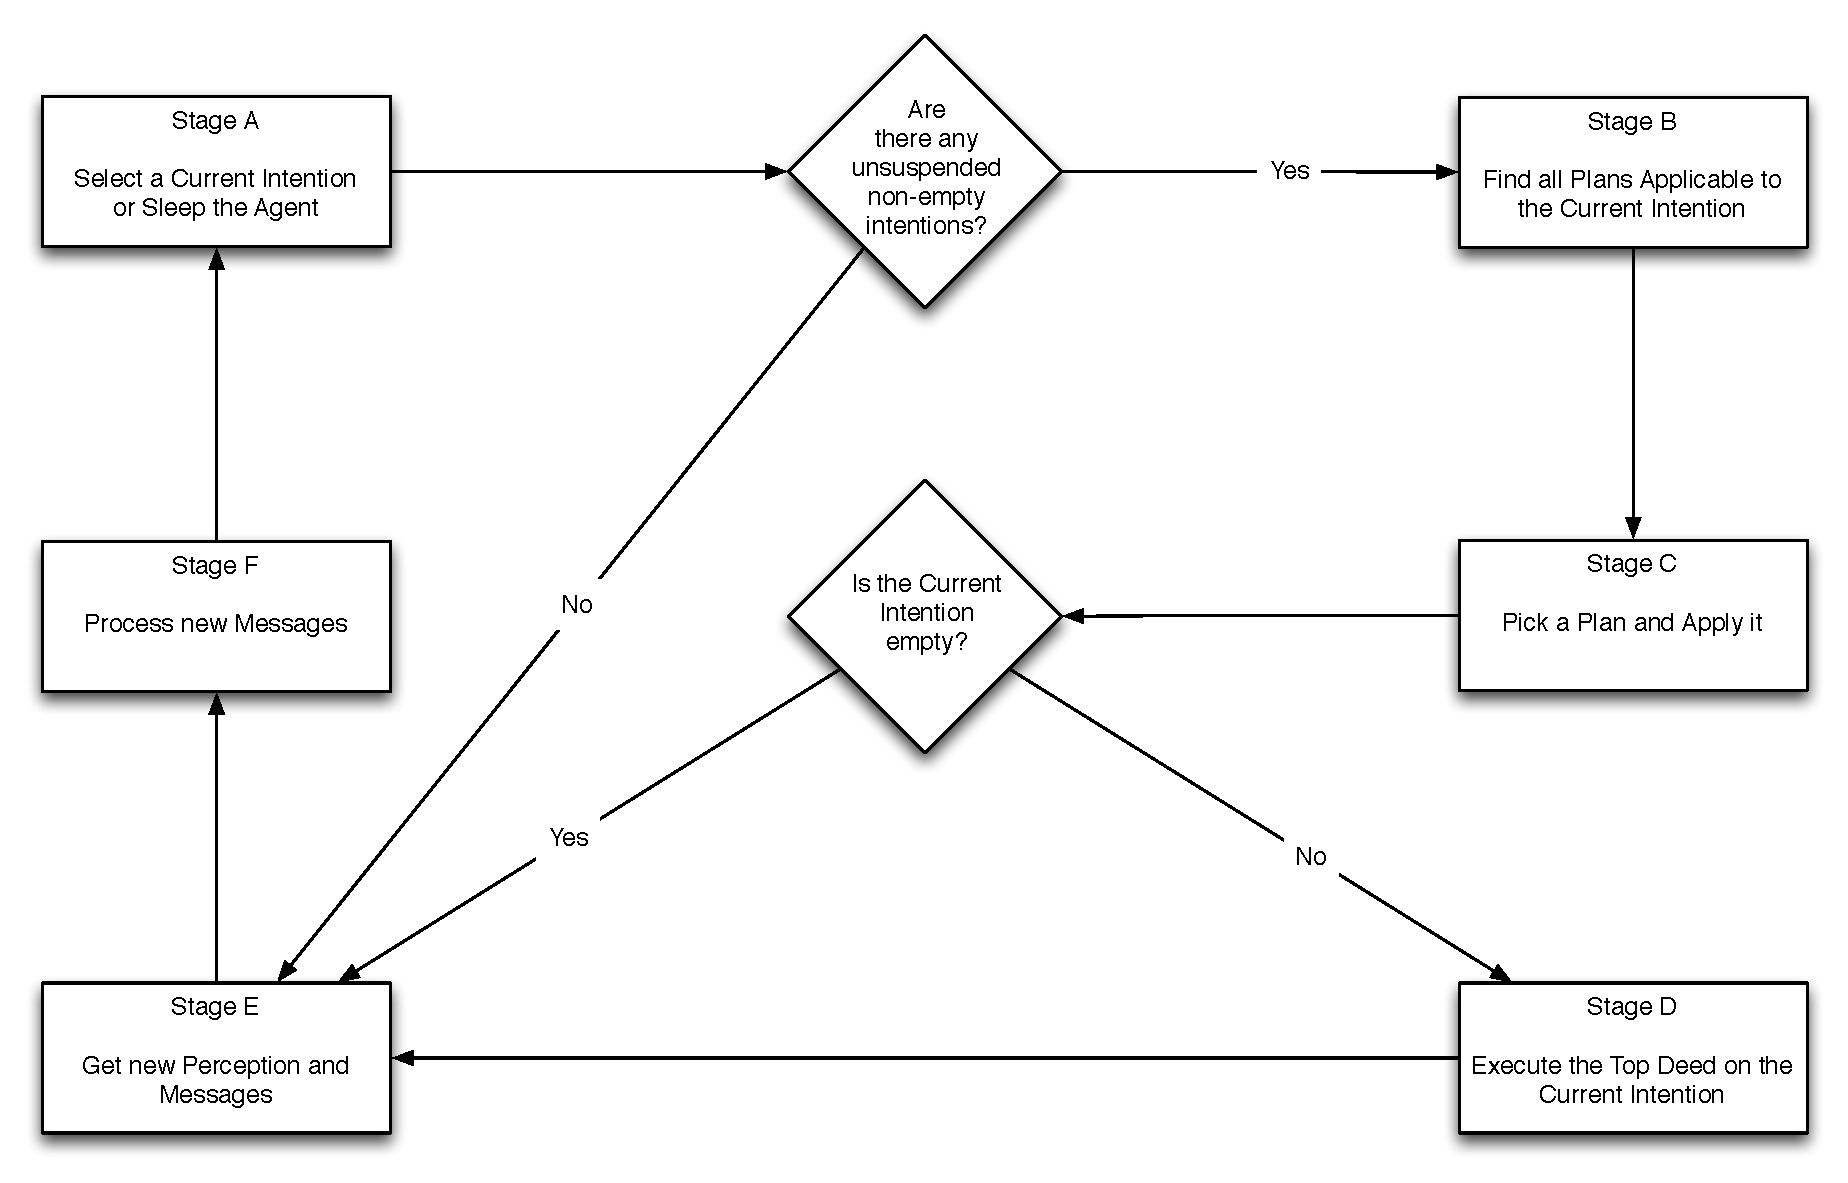
\includegraphics[width=\textwidth]{ReasoningCycle.pdf}
\caption{The \gwendolen\ Reasoning Cycle}
\label{fig:reasoning_cycle}
\end{figure}
\begin{description}
\item[Stage A]
A \gwendolen\ agent starts execution in stage A.  In this stage the agent selects an intention to be the current intention.  \gwendolen\ will rotates through the set of intentions ignoring any that are suspended until the current intention is locked in which case it will be reselected.  If there are no unsuspended intentions \gwendolen\ will sleep the agent.  In multi-agent contexts this means the agent will not do anything until \gwendolen\ detects that something has changed which may mean the agent now has something to do.  In single agent contexts the program stops when the agent sleeps.  At this stage \gwendolen\ also cleans up any empty intentions.
\item[Stage B]
The system generates all possible plans for the current intention - if the intention has already been planned then these are simply to continue processing the intention.  If the agent can't find a plan then it deletes the intention unless it has been triggered by a goal in which case it registers that there is a problem with the goal and generates a warning.
\item[Stage C]
\gwendolen\ has a list of plans.  It selects the first one in the list and applies it to the current intention.
\item[Stage D]
\gwendolen\ executes the top deed on the intention.  This might be taking an action, adding or removing a goal, adding or removing a belief, locking or unlocking the intention or suspending the intention using ``wait for''.
\item[Stage E]
\gwendolen\ requests that the agent's environment send it a list of \emph{percepts} (things the agent can detect) and messages.  The messages are stored for processing in the agent's inbox.  The percepts are compared with the agent's beliefs.  If a percept is new then an intention is created to add a belief corresponding to the percept.  If a previous percept can no longer be perceived then an intention is created to delete the belief.
\item[Stage F]
The agent sorts though its inbox and converts the messages into new intentions.
\end{description}

The actual code for the reasoning cycle can be found in \texttt{gwendolen.semantics.GwendolenRC}.  Each of the various rules that can be used in in a stage is a java class and they can all be found in the package \texttt{ail.semantics.operationalrules}.

\section{Using Java Debuggers to Debug \gwendolen\ programs}

Since the \gwendolen\ reasoning cycle is implemented in \java\ it is possible to use a \java\ debugger to debug \gwendolen\ programs.  In particular it can be useful to use a \java\ debugger to step through a \gwendolen\ program one stage of the reasoning cycle at a time watching to see how the state of the agent changes at each stage.

It is outside the scope of these tutorials to explain the use of \java\ debuggers.  There are many out there and one is built into most IDE's including Eclipse.

In our experience it is particularly useful when debugging in this way to place breakpoints in the \java\ \texttt{ail.semantics.AILAgent} class which is the generic class supporting agents in the Agent Infrastructure Layer (upon which \gwendolen\ is built).  In particular \texttt{ail.semantics.AILAgent} has a method called \texttt{reason} which controls looping through an agent's reasoning cycle.  We recommend placing such a break point either after \texttt{while(! RC.stopandcheck())} which is the top level loop through the reasoning cycle or at \texttt{rule.apply(this)} which is the moment that the outcome of a rule is calculated.

\paragraph{Exercise} Find a \java\ debugger (e.g., the one shipped with Eclipse) and discover how to set breakpoints using the debugger.  Set a breakpoint at \texttt{rule.apply(this)} in the \texttt{reason()} method in \texttt{ail.semantics.AILAgent} (you can find this in the \texttt{src/classes/ail/semantics} directory).  Run one of your programs with this breakpoint in place and see what happens and experiment in seeing what information you can discover about the agent state.

\section{Programming Exercise}


\end{document}
